\documentclass{report}


\usepackage{amsmath} % Better matrix environment
\usepackage{amssymb}
% \usepackage{enumitem}
\usepackage{etoolbox} % If conditions
\usepackage{graphicx}
\usepackage{listings} % for code
\usepackage{paralist} % inline numbering
\usepackage{caption}
\usepackage{subcaption}
\usepackage{tikz}
\usepackage{tikz-qtree,tikz-qtree-compat} % Trees
\usepackage{xkeyval}


% Squiggly lines
\usetikzlibrary{decorations.pathmorphing}


% Node shapes
\usetikzlibrary{shapes,decorations}

\newcommand{\VertexSet}{V}
\newcommand{\CellSet}{C}

\newcommand{\Visited}{V_{visited}}

% Cardinality of
\newcommand{\card}[1]{\left\vert{#1}\right\vert}

% powerset of
\newcommand{\powerset}[1]{\mathcal P \left({#1}\right)}



% Line that can go anywhere, structured region or outside
\tikzset{%
    anywhere/.style={
		decorate,
		decoration={
		    snake,
		    segment length=4,
		    amplitude=.9,post=lineto,
		    post length=2pt
		}
	}
}

% Line that can only go outside the structured region
\tikzset{outside/.style={dotted}}


% Ellipsis
\tikzset{ellipsis/.style={loosely dotted}}



\begin{document}

\chapter{Introduction}
Scientific computing is a large research branch touching on various areas in the scientific community as well as in various industries. An integral part of it is concerned with algorithms and techniques which operate on a mesh representation of a model, typically modelling physical phenomena such as the motion of fluids. SEE
% [Flow simulation and high performance computing, 1996a T. Tezduyar, http://www.tafsm.org/PUB_PRE/jALL/j63-CM96.pdf]
. SEE
% [http://www.sv.vt.edu/classes/MSE2094_NoteBook/97ClassProj/num/widas/history.html]
for a good introduction on finite element analysis.


Various methods of representing meshes exist, including X, Y, and Z
% [http://en.wikipedia.org/wiki/Polygon_mesh#Representations]
. Representations typically rely on encoding some form of explicitly-defined mapping between mesh elements. This can be represented straightforwardly as a flat array, with the array indices representing elements in the source set, and each value being one or more values representing one or more elements in the destination/target set. We focus our attention to the case where the number of target elements mapped to from each source element is constant. Such a map is known as a constant-arity map.

Consider for instance a quadrilateral mesh with two element sets \texttt{C} and \texttt{V}, representing the set of cells and vertices, respectively.
We can define a dat of coordinates, which associates the set each vertex $v \in V$ with a coordinate pair $(x_v, y_v)$, representing its position in 2D space.

We can then define an adjacency map (of constant arity 4) from cells to vertices:

\texttt{$C \rightarrow Node^4$}

Now consider an operation over this mesh, which performs a computation for each cell $c \in C$ as a function of its adjacent nodes ${n | n \in Map[c]}$, for instance computing the area of the cell. In particular consider the chain of memory access indirections and the resulting memory access patterns:

%
%             |   |             |   |
%             |   |  /----n3--->|   | -> (x_1, y_1)
%             |   | /           |   |
% cell_id ->  |   |/------n1--->|   | -> (x_4, y_4)
%             |   |\            |   |
%             |   | \-----n4--->|   | -> (x_5, y_5)
%             |   |  \          |   |
%             |   |   \---n2--->|   | -> (x_12, y_12)
%             |   |             |   |
%             |   |             |   |
%             |   |             |   |
%           cell2nodes         node2coordinate

Notice that proximate (or indded adjacent) nodes in the mesh need not exhibit a uniform memory access pattern. This is detrimental to performance for various reasons.
1. They do not exhibit spatial locality, a property which most modern CPU caches bank on to attain higher performance in IO bound applications, which may manifest through decisions regarding cache replacement strategies or data pre-fetching.
2. Looking up addresses, as opposed to computing them directly, will typically prohibit or limit the scope of compiler-performed optimizations, not least vectorizations.

Numerous strategies have been devoted to deal with this problem, notably applying a space filling curve to obtain a more favourable numbering, with closer elements tending to have closer numberings. While the space filling curve most certainly improves cache locality, it does not make use more obvious structure that may exist. A mesh that is irregular and unstructured on the whole may contain subregions of high regularity and uniform structure, whose regularity/uniformity may be locally exploitable in a more direct manner, for potentially higher gain!


We present Crystal mesh, a group of algorithms for \emph{extracting} regions of regularity in a mesh, reorganizing the mesh to \emph{expose} said structure in order to enable efficient \emph{exploitation}.
In particular, we present and evaluate an implementation for extracting and exposing structure in quadrilateral meshes on various examples, and evaluate a 33\% performance improvement achieved by exploiting the structure on the airfoil computation.


\chapter{Background}
\section{The mathematical mesh model}

Meshes often model physical objects and phenomena. This is typically achieved through the discretization of a continuous model, such as the surface or volume of an object, in order to approximate its physical properties to a desired degree of precision.
\par

The mesh model consists of a hierarchy of elements, which may include a subset the following:
\begin{itemize}
\item Polyhedra such as cubes or tetrahedrons
\item Polygons \emph{(also referred to as cells or faces)} such as triangles and quadrilaterals
\item Edges
\item Vertices \emph{(also referred to as nodes)}
\end{itemize}

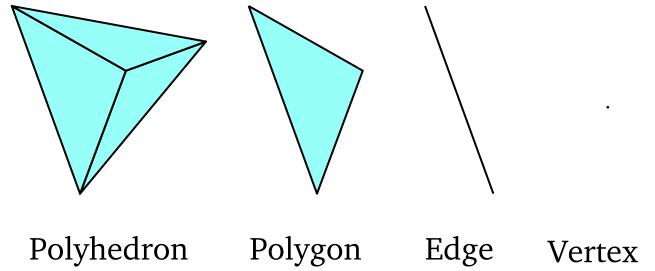
\includegraphics[scale=0.5]{images/background/mesh-elements.pdf}

Each element in the above hierarchy is built-up from those below it. Thus, a polyhedron is assimilated by a set of polygons, a polygon is composed by a set of edges, and an edge joins two vertices.


\subsection{Geometry vs topology}
There is a key distinction to make between the geometric and topological properties of a mesh.

Since meshes model a physical reality, the elements of a mesh may be spatially embedded: vertices are associated with points in space, and edges are formed as segments joining their two vertices. This affects \emph{geometric} properties of the mesh, such as its surface area or volume.

On the other hand, the hierarchy of elements described above induces a mesh topology. This describes the connectedness of the mesh, that is to say how elements relate to one another. For instance, we may describe two vertices sharing an edge as \emph{adjacent}, or two cells being \emph{incident} on an edge.
\par
In this work we concern ourselves solely with the topological structure of meshes, treating its geometry as arbitrary data that is associated with its respective elements (the position of a vertex for instance). Figure~\ref{fig:same-topology} illustrates the difference between the two concepts.

\begin{figure}
    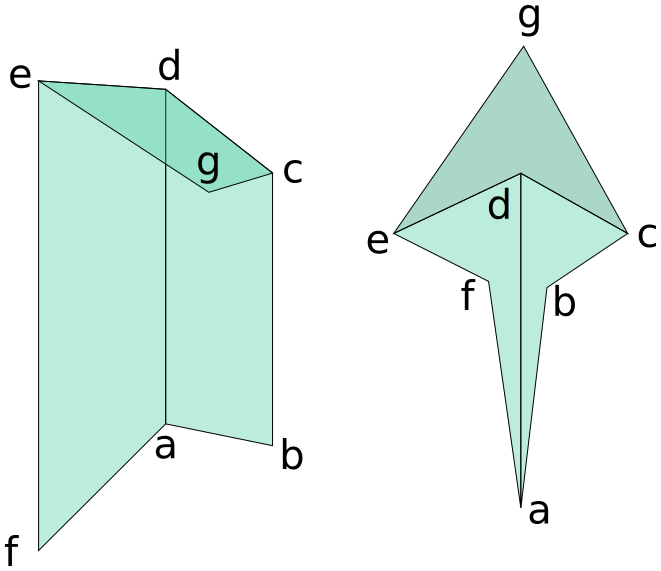
\includegraphics[scale=0.5]{images/background/same-topology.pdf}
    \caption{Despite having completely different geometric shapes and properties, the two meshes are topologically equivalent. The labels indicate corresponding vertices.}
    \label{fig:same-topology}
\end{figure}




\subsection{Manifold meshes}
A mesh is a manifold if the following properties hold:
\begin{enumerate}
\item All edges are adjacent to either one or two faces.

\item All faces meeting at a given vertex must form either an open or a closed fan around that vertex (Figure~\ref{fig:open-closed-fans}).
\end{enumerate}

% Open and closed fans
\begin{figure}
    \sidebyside
        {\includegraphics[scale=0.2]{images/background/closed-fan.pdf}
        \caption{A closed fan}}
        {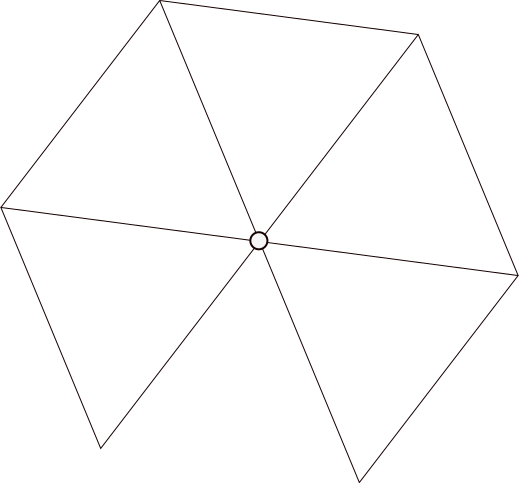
\includegraphics[scale=0.2]{images/background/open-fan.pdf}
        \caption{An open fan}}
    \caption{}
    \label{fig:open-closed-fans}
\end{figure}

Figure~\ref{fig:non-manifolds} demonstrates examples of non-manifold meshes.

% Non-manifolds
\begin{figure}
    \sidebysidefour
    {\includegraphics[scale=0.2]{images/background/bad-fan.pdf}
        \caption{Faces incident on a vertex which do not form a continuous fan}}
    {\includegraphics[scale=0.2]{images/background/bad-fan2.pdf}
        \caption{An extra face that breaks off from the otherwise closed fan}}
    {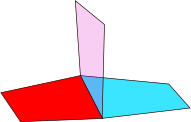
\includegraphics[scale=0.8]{images/background/bad-multi-edge.pdf}
        \caption{More than two faces incident on a single edge}}
    {\includegraphics[scale=0.8]{images/background/bad-no-edge.pdf}
        \caption{An edge with no incident faces}}

    \caption{Examples of non-manifold meshes.}
    \label{fig:non-manifolds}
\end{figure}

In this work we consider manifold meshes exclusively, and future mentions of `mesh' shall implicitly refer to manifold meshes.




\section{The mesh data structure}

We describe how a mesh model is manifest at the data structure level. There are three general component types can be identified:
\begin{itemize}
\item Entity sets
\item Associative data
\item Relations between two entity sets
\end{itemize}

In the following sections, the examples shall refer to the mesh depicted in figure~\ref{fig:example-mesh}.

\begin{figure}
    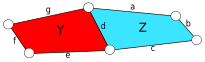
\includegraphics[scale=2]{images/background/mesh-data-structure.pdf}
    \caption{Example mesh with labelled elements.}
    \label{fig:example-mesh}
\end{figure}


\subsection{Entity sets}
Each set represents a certain type of entity in the mesh, such as vertices or cells. Each element in a set is associated with a unique identifier. Integers are a common choice as an identifier for a couple of reasons:
\begin{itemize}
\item They need not be enumerated explicitly. All we need is the set cardinality and a starting index.
\item They are convenient for direct-indexed array accesses, as well as for more general indexing methods.
\end{itemize}

See figure~\ref{fig:entity-sets} for examples.

\begin{figure}
    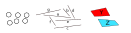
\includegraphics[scale=4]{images/background/entity-sets.pdf}
    \caption{The entity sets of the mesh in figure~\ref{fig:example-mesh}. These are (from left to right) the vertices, edges, and cells.}
    \label{fig:entity-sets}
\end{figure}


\subsection{Associative data}
Arbitrary data which is associated with elements of a particular entity set. For instance, spatial coordinates associated with each vertex. A typical representation is a flat array indexed by element identifier.
This is the data over which we perform our computations and ultimately care about. Everything else is incidental.

See figure~\ref{fig:associative-data} for an example.

\begin{figure}
    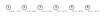
\includegraphics[scale=4]{images/background/associative-data.pdf}
    \caption{Coordinate data associated with the vertices of the mesh in figure~\ref{fig:example-mesh}.}
    \label{fig:associative-data}
\end{figure}


\subsection{Relation maps between two entity sets}
Entity sets may have relations defined between them, a mapping from an element in a source set to one or more corresponding elements in the destination set. For instance, we may have an adjacency relation from the vertex set to itself, or an inclusion relation from the cell set to the vertex set.
In a general unstructured mesh these relations must be explicitly stored, typically as an array indexed by the source element's identifier.

See figure~\ref{fig:relation} for an example.

\begin{figure}
    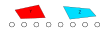
\includegraphics[scale=4]{images/background/relation.pdf}
    \caption{Inclusion relation from cells to vertices, as depicted in the mesh of figure~\ref{fig:example-mesh}.}
    \label{fig:relation}
\end{figure}




\section{The mesh core-computation contract}
Given a mesh model and its underlying representation, computation logic provided by an external user is to be executed. We refer to this as the \emph{core-computation}; this is to disambiguate it from other incidental processing, such as structure detection.
Our contract to the user is described in what follows.

\subsection{Given: entity set}
We are given an entity set over which to operate, for example the set of edges or the set of cells. The core-computation consists of executing a computation for each element of this set. This is analogous to the \emph{map} phase of the MapReduce programming model\footnote{REFERENCE}, though we restrict our usage of the term \emph{map} to refer to relation maps.

\subsection{Given: relation-map tree}
We are given a tree structure defining which relation maps to use and how to access them. This is best explained through an example, illustrated in figure~\ref{fig:relation-tree}.


\begin{figure}
    %% Key icon
    \newcommand{\keyicon}{
\includegraphics[width=6pt]{images/background/key.pdf}}

    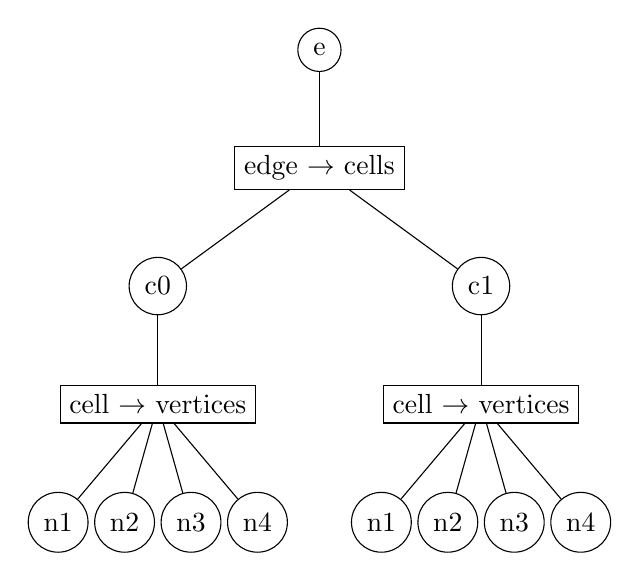
\begin{tikzpicture}[every tree node/.style={draw,circle},
        level distance=1.5cm,
        edge from parent path={(\tikzparentnode) -- (\tikzchildnode)}]

    \tikzset{level 2/.style={sibling distance=0.8cm}}

    \Tree
    [.{e}
        \edge node[auto=right] {\keyicon};
        [.\node[rectangle] {edge $\rightarrow$ cells};
            [.{c0}
                \edge node[auto=right] {\keyicon};
                [.\node[rectangle] {cell $\rightarrow$ vertices};
                    [.n1 ]
                    [.n2 ]
                    [.n3 ]
                    [.n4 ]
                ]
            ]
            [.{c1}
                \edge node[auto=right] {\keyicon};
                [.\node[rectangle] {cell $\rightarrow$ vertices};
                    [.n1 ]
                    [.n2 ]
                    [.n3 ]
                    [.n4 ]
                ]
            ]
        ]
    ]
    \end{tikzpicture}
    \caption{EXPLANATION}
    \label{fig:relation-tree}
\end{figure}





% \item The entity set over which to operate.
% \item Any relation maps to follow, and the variables by which they are indexed. Indexing variables may include the current iteration element, as well as the targets got by following another map.
% In general this may involve complex chains of maps, though only up to to two levels of indirection are used in practice.
% \item A kernel function which is to be applied to each element in the given entity set.
% \end{itemize}

A \emph{kernel function} specifying the computation logic is given. This kernel function is associated with a particular entity set.

The execution contract

When performing some computation over a mesh, the data access pattern followed is typically as follows:
\begin{enumerate}
\item Iterate over the elements of an entity set, in no particular order.
\item For each element iterated over, gather any handles to associated elements (the indices of adjacent elements, say). This may involve handles obtained through a chain of set relationship maps.
\item Access the associative data using the gathered handles.
\end{enumerate}


 The computation is often specified as a \emph{kernel function} operating a particular entity set



\chapter{Diving into the problem}

\section{A basic definition of structure}
What we would like is a form of structure which is
\begin{enumerate*}[label=\alph*)]
\item representable as a data structure, and \item efficient in terms of performance.
\end{enumerate*}

Given our semantic knowledge about the mesh model we can ascertain some facts about relationship maps:
\begin{itemize}
\item They are sparse: element arity is very small compared to the number of elements, and is in fact unrelated to it.
\item They have a high clustering coefficient: Relationships tend to be localized, forming tightly connected clusters.
% TODO REFERENCE TO CLUSTERING COEFFICIENTS
\end{itemize}

These properties arise as a consequence of meshes modelling real-world phenomena that exist in a Cartesian space.
On this basis, we consider a spatial embodiment of element relationships, organising the elements in a discrete space such that the uniform relationship is apparent.

Bear in mind that this approach carries no relation to any geometric data associated with elements, such as the coordinates of vertices. To make this distinction clear, as well as to emphasize its discrete nature, we address this Cartesian-like space by rows and columns rather than x and y coordinates.

\subsection{Example: Naca0012 mesh}
Below is a small extract from the NACA0012 mesh\footnote{Thanks to Dr. Peter Vincent, George Ntemos and Harry Davis}, showing the cross section of an aerofoil mesh and its interaction with surrounding fluid. The mesh is divided into cells which represent the ...

\newcommand{\drawnaca}[2]{
	% trim left bottom right top
	\includesvg[svgpath=#1]{#2}
}
\drawnaca{images/defining-structure/}{naca0012-plain}

The vertices in the highlighted region seem like good candidates for a ``structured region'', forming a two-dimensional lattice in a discrete Cartesian space. This ``structured region'' has the properties outlined below.

\subsection{Properties of a structured region}
\label{sec:structured-region-properties}
\begin{enumerate}
\item All vertices have a uniform arity of four.
\item Every vertex has a consistent discrete direction (for example the cardinal directions: north east, south, west) with respect to the other vertices. In other words, the direction is transitive: if vertex $a$ is above vertex $b$, and vertex $b$ is above vertex $c$, then vertex $a$ is above vertex $c$. As a non-example, consider this case:
** INSERT IMAGE AND EXPLANATION **
\end{enumerate}


\drawnaca{images/defining-structure/}{naca0012-node-structure}

%% TODO Maybe not introduce data structure yet????
We can propagate this inherent structure from the mesh model to the underlying data structure, representing this two-dimensional lattice using a two-dimensional array. Vertices may be assigned Cartesian coordinates, but in spirit of the space's discreteness we shall use rows and columns instead.

\drawnaca{images/defining-structure/}{naca0012-node-grid}


\newcommand{\strV}{V_{str}}
\newcommand{\adjstrV}{V_{adjstr}}
\newcommand{\AdjVVstr}{Adj_{\adjstrV\strV}}

Let us call $\VertexSet$ the set of all vertices, and $\strV \subseteq \VertexSet$ the set of vertices in the ``structured region''.

\subsection{Representing the vertex-vertex adjacency}

Now consider the vertex-vertex adjacency relation $\AdjVV: \VertexSet \mapsto \VertexSet$ in context of the ``structured region'' $\strV$. We can directly locate a particular neighbour of any vertex, for example its north neighbour, so long as that neighbour is also within the structured region. This restricts the set of vertices with fully-accessible neighbours to those which are not on the borders of the ``structured region''. This is the subset of vertices $\adjstrV \subseteq \strV$ which are structured \emph{with respect to} $\AdjVV$. This induces a new relation which operates purely within the structured region:
$$\AdjVVstr: \adjstrV \mapsto \strV$$

\drawnaca{images/defining-structure/}{naca0012-node-neighbours}


\definecolor{neighbourstructurecolor}{RGB}{174,190,226}

% Draw structured node region
\begin{tikzpicture}[scale=0.7]
	\newcommand{\stylewithfill}[1]{\tikzstyle{every node}=[draw, shape=circle, minimum size=0.8cm, fill=#1];}
	\stylewithfill{none}

	% ROW 0
	\drawgrid{rows=1, cols=3, rowoffset=0, coloffset=4, labeler=\plainlabelnode, labelerA=0, labelerB=2,
		southborder=structured}

	% ROW 1
	\drawgrid{rows=1, cols=2, rowoffset=-2, coloffset=0, labeler=\plainlabelnode, labelerA=1, labelerB=0,
		eastborder=structured}

	{
	\stylewithfill{neighbourstructurecolor}
	\drawgrid{rows=1, cols=2, rowoffset=-2, coloffset=4, labeler=\plainlabelnode, labelerA=1, labelerB=2,
		northborder=structured, southborder=structured, westborder=structured, eastborder=structured}
	}

	\drawgrid{rows=1, cols=1, rowoffset=-2, coloffset=8, labeler=\plainlabelnode, labelerA=1, labelerB=4,
		northborder=structured, southborder=structured, westborder=structured}


	\drawgrid{rows=1, cols=1, rowoffset=-2, coloffset=12, labeler=\plainlabelnode, labelerA=1, labelerB=6,
		southborder=structured, eastborder=structured}

	\drawgrid{rows=1, cols=1, rowoffset=-2, coloffset=14, labeler=\plainlabelnode, labelerA=1, labelerB=7,
		westborder=structured}

	% ROW 2
	\drawgrid{rows=1, cols=1, rowoffset=-4, coloffset=4, labeler=\plainlabelnode, labelerA=2, labelerB=2,
		northborder=structured, southborder=structured, eastborder=structured}

	{
	\stylewithfill{neighbourstructurecolor}
	\drawgrid{rows=1, cols=2, rowoffset=-4, coloffset=6, labeler=\plainlabelnode, labelerA=2, labelerB=3,
		northborder=structured, southborder=structured, eastborder=structured, westborder=structured}
	}

	\drawgrid{rows=1, cols=1, rowoffset=-4, coloffset=10, labeler=\plainlabelnode, labelerA=2, labelerB=5,
		southborder=structured, westborder=structured, eastborder=structured}

	\drawgrid{rows=1, cols=1, rowoffset=-4, coloffset=12, labeler=\plainlabelnode, labelerA=2, labelerB=6,
		northborder=structured, westborder=structured}

	% ROW 3
	\drawgrid{rows=1, cols=1, rowoffset=-6, coloffset=4, labeler=\plainlabelnode, labelerA=3, labelerB=2,
		northborder=structured, southborder=structured, eastborder=structured}

	{
	\stylewithfill{neighbourstructurecolor}
	\drawgrid{rows=1, cols=2, rowoffset=-6, coloffset=6, labeler=\plainlabelnode, labelerA=3, labelerB=3,
		northborder=structured, southborder=structured, eastborder=structured, westborder=structured}
	}

	\drawgrid{rows=1, cols=1, rowoffset=-6, coloffset=10, labeler=\plainlabelnode, labelerA=3, labelerB=5,
		northborder=structured, westborder=structured}

	% ROW 4
	\drawgrid{rows=1, cols=1, rowoffset=-8, coloffset=2, labeler=\plainlabelnode, labelerA=4, labelerB=1, eastborder=structured}

	{
	\stylewithfill{neighbourstructurecolor}
	\drawgrid{rows=1, cols=2, rowoffset=-8, coloffset=4, labeler=\plainlabelnode, labelerA=4, labelerB=2,
		northborder=structured, southborder=structured, eastborder=structured, westborder=structured}
	}

	\drawgrid{rows=1, cols=1, rowoffset=-8, coloffset=8, labeler=\plainlabelnode, labelerA=4, labelerB=4,
		northborder=structured, westborder=structured}

	% ROW 5
	\drawgrid{rows=1, cols=2, rowoffset=-10, coloffset=4, labeler=\plainlabelnode, labelerA=5, labelerB=2,
		northborder=structured}
\end{tikzpicture}

The key insight we make is that for structured regions in a mesh we need not represent set relationship maps explicitly; the uniformity of set relations allows us to deduce the relationships. We can encode the relation $\AdjVVstr$ very simply. Given a vertex $n_{r,c} \in \adjstrV$, located at row $r$ and column $c$, its four vertex neighbours are $n_{r,c-1}$, $n_{r,c+1}$, $n_{r-1,c}$, and $n_{r+1,c}$.



% Draw structured node region
\begin{tikzpicture}[scale=1]
	\newcommand{\stylewithfill}[1]{\tikzstyle{every node}=[draw, shape=circle, minimum size=1.3cm, fill=#1];}
	\stylewithfill{none}

	% ROW 0
	\drawgrid{rows=1, cols=1, rowoffset=0, coloffset=2,
		labeler=\varlabelnode, labelerA=-1, labelerB=0, labelerC=r, labelerD=c,
		southborder=structured}

	% ROW 1
	\drawgrid{rows=1, cols=1, rowoffset=-2, coloffset=0,
		labeler=\varlabelnode, labelerA=0, labelerB=-1, labelerC=r, labelerD=c,
		eastborder=structured}

	{
		\stylewithfill{neighbourstructurecolor}
		\drawgrid{rows=1, cols=1, rowoffset=-2, coloffset=2,
			labeler=\varlabelnode, labelerA=0, labelerB=0, labelerC=r, labelerD=c,
			eastborder=structured, westborder=structured, northborder=structured, southborder=structured}
	}

	\drawgrid{rows=1, cols=1, rowoffset=-2, coloffset=4,
		labeler=\varlabelnode, labelerA=0, labelerB=1, labelerC=r, labelerD=c,
		westborder=structured}

	% ROW 2
	\drawgrid{rows=1, cols=1, rowoffset=-4, coloffset=2,
		labeler=\varlabelnode, labelerA=1, labelerB=0, labelerC=r, labelerD=c,
		northborder=structured}

\end{tikzpicture}


\section{Mesh structure as a data structure}
The choice of data structure to represent the structured region is a key one, touching on various aspects:
\begin{itemize}
\item Scope of structure representation: what level of structure can be represented.
\item Implementation complexity of structure detection: how complex a detection algorithm is required.
\item Runtime performance of structure detection: the time and space complexity of the detection algorithm.
\item Storage requirements for detected structure: the storage requirements for the detected structure.
\item Runtime performance of computation over the structured region.
\end{itemize}

We analyse several possible data structure representations.

\subsection{Structure bit map}

\newcommand{\drawbitmap}[2]{
	% trim left bottom right top
	\includesvg[svgpath=#1]{#2}
}

Represent the bounding box around the structured region as a two-dimensional bit map, with each bit representing a vertex position in the superimposed grid. An \emph{on} bit indicates that the corresponding vertex is part of the structured region, an \emph{off} bit otherwise.

\drawbitmap{images/bitmap-representation/}{plain-bitmap}

A bit map can represent \emph{any} structured region which adheres to the properties listed in section~\ref{sec:structured-region-properties}. They are very flexible, capable of representing complex formations as well as handling small anomalies in structure.

Let us define the \emph{efficiency} $\epsilon$ of a bit map as the percentage of its bits which are \emph{on}, as the \emph{off} bits represent wasted vertices. Bit maps with high $\epsilon$ are favourable for several reasons:
\begin{itemize}
\item \emph{Off} bits increase the storage space of the structured region, up to $O(\card{\VertexSet})$ in the worst case, as opposed to $O(\card{STRUCTURED VERTICES})$.
\item \emph{Off} bits similarly worsen the runtime performance, again up to $O(\card{\VertexSet})$ due to wasted execution.
\end{itemize}

A detection algorithm would likely be implemented using a variant of a general graph search algorithm such as breadth-first search or depth-first search. Further consolidation work may be needed to compact disconnected structured components in order to maximize $\epsilon$.
\drawbitmap{images/bitmap-representation/}{disjoint-bitmap}
\drawbitmap{images/bitmap-representation/}{disjoint2-bitmap}



\subsection{Row-specific boundaries}

Represent the structured region as a sequence of consecutive fixed-length rows, permitting vertices outside the structured region to cluster at the beginning and ends of each row. A structured region is then represented by the row-length, as well as individual begin and end offsets for each row.

\drawbitmap{images/per-row-representation/}{plain-per-row}

Storing row-specific boundaries reduces the storage requirement by the order of row-length times.
No executions are wasted as the loop iterations are constrained to vertices in the structured region.
A detection algorithm can be implemented as a simple row-by-row traversal in linear time and space.


On the downside, this scheme trades some of the flexibility offered by the bit map representation, in particularly anomalies in structure which do not occur at the boundaries.


\subsection{Full rectangle}

Represent the structured region as a rectangle of given length and width, with all elements corresponding strictly to vertices within the structured region. The structured region is thus simply represented by the length and the width: the number of rows and the number of columns.

The storage requirement is now constant with respect to the size of the structured region.
Loop iterations are fixed for each region, enabling further optimisation opportunities.
A detection algorithm, as above, can be implemented as a simple row-by-row traversal.

On the downside, the scope of structure representable is limited, being only capable of representing rectangles proper.


\chapter{Structure Extraction}
\newcommand{\Structured}{V_{structured}}
\newcommand{\AdjVV}{Adj_{\VertexSet\VertexSet}}
\newcommand{\vinit}{v_{init}}



\subsection{Inputs}
\begin{enumerate}
\item A non-reflexive and symmetric vertex-vertex adjacency relation:
$$ \AdjVV: \VertexSet \mapsto \powerset{\VertexSet} $$

\item A set of visited vertices
$$ \Visited \subseteq \VertexSet $$

\item An unvisited start vertex
$$ \vinit \in \VertexSet \setminus \Visited $$
\end{enumerate}


\subsection{Outputs}
\begin{enumerate}
\item A structured set of vertices $\Structured \subseteq \VertexSet \setminus \Visited $ forming the extracted structured region.
The vertices $\Structured$ are structured on a 2-dimensional Cartesian lattice with $m$ rows and $n$ columns.
\end{enumerate}


%%%% PHASE 1

%% Phase 1 summary
\subsection{Phase 1: Grow a quad}
Starting from the initial vertex $\vinit$, call it $n_{1,1}$, we would like to discover three other vertices $n_{1,2}$, $n_{2,1}$, and $n_{2,2}$ that, together with $n_{1,1}$, form a quad in a structured quad region. They must satisfy the following constraints:

\begin{itemize}
\item Each of the four vertices must have exactly 4 neighbours.
\item Each of the following pairs of vertices are neighbours: $n_{1,1}$~and~$n_{1,2}$ ; $n_{1,2}$~and~$n_{2,2}$ ; $n_{2,2}$~and~$n_{2,1}$ ; $n_{2,1}$~and~$n_{1,1}$.
\item Each of the vertices must \emph{not} neighbour any vertex that is part of the structured region thus far, apart from those vertices explicitly mentioned.
\end{itemize}

%% Phase 1 diagram

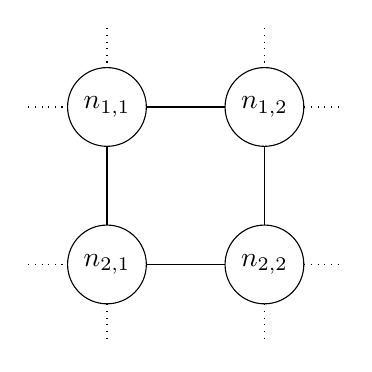
\begin{tikzpicture}[scale=1]
		% Default action for each node
		\tikzstyle{every node}=[draw, shape=circle, minimum size=1cm];

											\coordinate (northleft) at (0, 2);	\coordinate (northright) at (2, 2);
		\coordinate (westup) at (-1,1);		\node (r1c1) at (0,1) {$n_{1,1}$};	\node (r1c2) at (2,1) {$n_{1,2}$};	\coordinate (eastup) at (3,1);
		\coordinate (westdown) at (-1,-1);	\node (r2c1) at (0,-1) {$n_{2,1}$};	\node (r2c2) at (2,-1) {$n_{2,2}$};	\coordinate (eastdown) at (3,-1);
											\coordinate (southleft) at (0, -2);	\coordinate (southright) at (2, -2);

		% Horizontals
		\draw[outside] (westup) -- (r1c1);
		\draw (r1c1) -- (r1c2);
		\draw[outside] (r1c2) -- (eastup);

		\draw[outside] (westdown) -- (r2c1);
		\draw (r2c1) -- (r2c2);
		\draw[outside] (r2c2) -- (eastdown);

		% Verticals
		\draw[outside] (northleft) -- (r1c1);
		\draw (r1c1) -- (r2c1);
		\draw[outside] (r2c1) -- (southleft);

		\draw[outside] (northright) -- (r1c2);
		\draw (r1c2) -- (r2c2);
		\draw[outside] (r2c2) -- (southright);
	\end{tikzpicture}

%% Phase 1 algorithm

\subsubsection{Algorithm}

\begin{enumerate}
\item If $\vinit$ does not have exactly 4 neighbours, that is $ \card{\AdjVV(\vinit)} \neq 4 $, return immediately with $\Structured = \varnothing$.
\item Let $ n_{1,1} = \vinit $, and let $ a, b, c \in \AdjVV(\vinit) $ be distinct vertex neighbours of $\vinit$. Consider vertices $a$ and $b$. If they do not both have exactly 4 neighbours, then they cannot form a part of a structured quad region. Return immediately with $\Structured = \varnothing$.

\item Otherwise, there are three cases:

	%%%% BEGIN THREE CASES
	\begin{enumerate}[label=Case \alph*)]

	%% Straight line case
	\item $a$ and $b$ have exactly one neighbour in common, which must be $n_{1,1}$ by construction, expressed by:
	$$ \card{\AdjVV(a) \cap \AdjVV(b)} = 1$$
	$a, n_{1,1}, b $ are \emph{topologically} along a straight line of a structured grid, and hence cannot form a quad.
	We therefore consider $b$, $n_{1,1}$, and  $c$ instead as candidates, letting $n_{2,1} = b$ and $n_{1,2} = c$.
	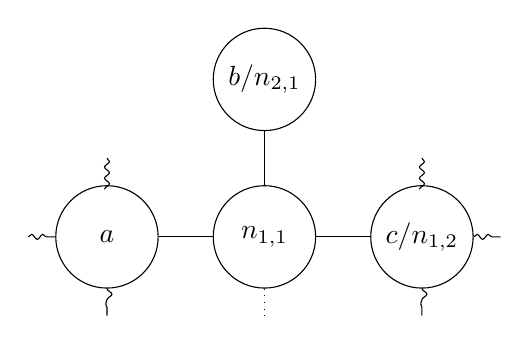
\begin{tikzpicture}
		% Default action for each node
		\tikzstyle{every node}=[draw, shape=circle, minimum size=1.3cm];

										\coordinate (northleft) at (-1,2);	\node (b) at (1,3) {$b / n_{2,1}$};	\coordinate (northright) at (3,2);
		\coordinate (west) at (-2,1);	\node (a) at (-1,1) {$a$};			\node (n11) at (1,1) {$n_{1,1}$};	\node (c) at (3,1) {$c / n_{1,2}$};	\coordinate (east) at (4,1);
										\coordinate (southleft) at (-1,0);	\coordinate (southmid) at (1,0);	\coordinate (southright) at (3,0);

		\draw[anywhere] (west) -- (a);
		\draw (a) -- (n11) -- (c);
		\draw[anywhere] (c) -- (east);

		\draw[anywhere] (northleft) -- (a) -- (southleft);
		\draw (b) -- (n11);
		\draw[outside] (n11) -- (southmid);
		\draw[anywhere] (northright) -- (c) -- (southright);
	\end{tikzpicture}


	%% Angle case
	\item $a$ and $b$ have exactly two neighbours in common, one of which must be $n_{1,1}$ by construction, expressed by:
	$$ \card{\AdjVV(a) \cap \AdjVV(b)} = 2$$
	We continue with vertices $a$, $n_{1,1}$, and $b$ as candidates, letting $n_{2,1} = a$ and $n_{1,2} = b$.
	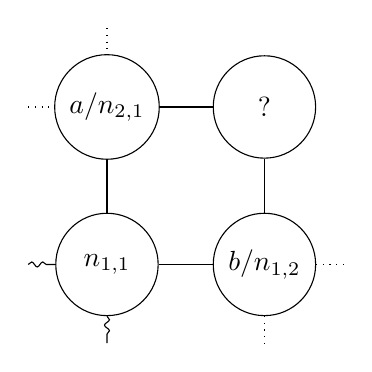
\begin{tikzpicture}
		% Default action for each node
		\tikzstyle{every node}=[draw, shape=circle, minimum size=1.3cm];

											\coordinate (northleft) at (-1,4);		\coordinate (northright) at (1,4);
		\coordinate (westup) at (-2,3);		\node (a) at (-1,3) {$a / n_{2,1}$};	\node (d) at (1,3) {$?$};			\coordinate (eastup) at (2,3);
		\coordinate (westdown) at (-2,1);	\node (n11) at (-1,1) {$n_{1,1}$};		\node (b) at (1,1) {$b / n_{1,2}$};	\coordinate (eastdown) at (2,1);
											\coordinate (southleft) at (-1,0);		\coordinate (southright) at (1,0);



		\draw[outside] (westup) -- (a);
		\draw (a) -- (d);
		% \draw (d) -- (eastup);

		\draw[anywhere] (westdown) -- (n11);
		\draw (n11) -- (b);
		\draw[outside] (b) -- (eastdown);

		\draw[outside] (northleft) -- (a);
		\draw (a) -- (n11);
		\draw[anywhere] (n11) -- (southleft);

		% \draw (northright) -- (d);
		\draw (d) -- (b);
		\draw[outside] (b) -- (southright);

	\end{tikzpicture}


	\item $a$ and $b$ have more than two neighbours in common\footnote{note that the set is non-empty by construction}, expressed by:
	$$ \card{\AdjVV(a) \cap \AdjVV(b)} > 2$$
	We cannot form a quad, and hence return immediately with $\Structured = \varnothing$.

	\end{enumerate}
	%%%% END THREE CASES

\item Find the common neighbours of $n_{2,1}$ and $n_{1,2}$. If there are not exactly two neighbours, return immediately with $\Structured = \varnothing$.

\item One of the two neighbours must be $n_{1,1}$ by construction. Let the other neighbour be $n_{2,2}$

\item Let $N = \{ n_{1,1}, n_{1,2}, n_{2,1}, n_{2,2} \}$. If any vertex $n \in N$ is in $\Visited$, that is $N \cap \Visited \neq \varnothing$, then return immediately with $\Structured = \varnothing$. Otherwise add the vertices in $N$ to $\Visited$.

\item Ensure for every vertex $n \in N$ that its visited neighbours, $\AdjVV(n) \cap \Visited$, are exactly those explicitly stated above. If this is not the case, remove $N$ from $\Visited$ and return immediately with $\Structured = \varnothing$.

\item Set $\Structured = \{ n_{1,1}, n_{1,2}, n_{2,1}, n_{2,2} \}$, and continue to the next phase.

The structured region looks as follows thus far.
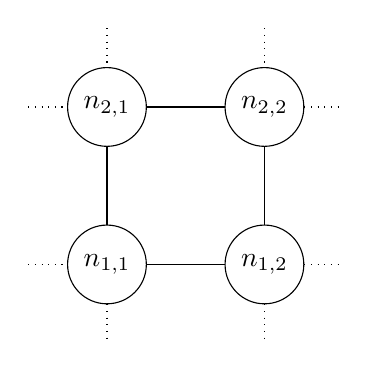
\begin{tikzpicture}
	% Default action for each node
	\tikzstyle{every node}=[draw, shape=circle, minimum size=1cm];

										\coordinate (northleft) at (-1,4);	\coordinate (northright) at (1,4);
	\coordinate (westup) at (-2,3);		\node (n21) at (-1,3) {$n_{2,1}$};	\node (n22) at (1,3) {$n_{2,2}$};	\coordinate (eastup) at (2,3);
	\coordinate (westdown) at (-2,1);	\node (n11) at (-1,1) {$n_{1,1}$};	\node (n12) at (1,1) {$n_{1,2}$};	\coordinate (eastdown) at (2,1);
										\coordinate (southleft) at (-1,0);	\coordinate (southright) at (1,0);



	\draw[outside] (westup) -- (n21);
	\draw (n21) -- (n22);
	\draw[outside] (n22) -- (eastup);

	\draw[outside] (westdown) -- (n11);
	\draw (n11) -- (n12);
	\draw[outside] (n12) -- (eastdown);

	\draw[outside] (northleft) -- (n21);
	\draw (n21) -- (n11);
	\draw[outside] (n11) -- (southleft);

	\draw[outside] (northright) -- (n22);
	\draw (n22) -- (n12);
	\draw[outside] (n12) -- (southright);

\end{tikzpicture}

\end{enumerate}




\end{document}
